\graphicspath{ {./images/1_Overview} }
\newpage

\section{Overview}
\subsection{Background}
GlycoDash is an R Shiny dashboard created for processing mass spectrometry data obtained from LaCyTools, SweetSuite or Skyline.
The data is uploaded to the dashboard and optionally merged with metadata.
Spectral curation and analyte curation are then performed to exclude data that is of insufficient quality from further analysis.
Total area normalization is performed on the curated glycopeptide data per glycosylation site.
GlycoDash then offers the options to calculate glycosylation traits, quantify proteins, determine glycosylation site occupancies, assess the repeatability of technical replicates, and to perform simple data visualizations.

The output data is a file in \texttt{.xlsx} format that can be easily imported into software such as RStudio or SPSS for further data analysis.
A processing report in HTML format can also be downloaded.
By listing all choices that were made, this file ensures the reproducibility of all processing steps.

For background information about GlycoDash, please refer to \href{https://doi.org/10.1007/s00216-025-05794-3}{our publication}.
GlycoDash has undergone continued development and refinement since this paper was published.
The current version includes additional features and improvements that extend beyond the scope of the published manuscript.


\subsection{User interface}
When launching GlycoDash, you will be presented with the page shown below. 

\begin{center}
	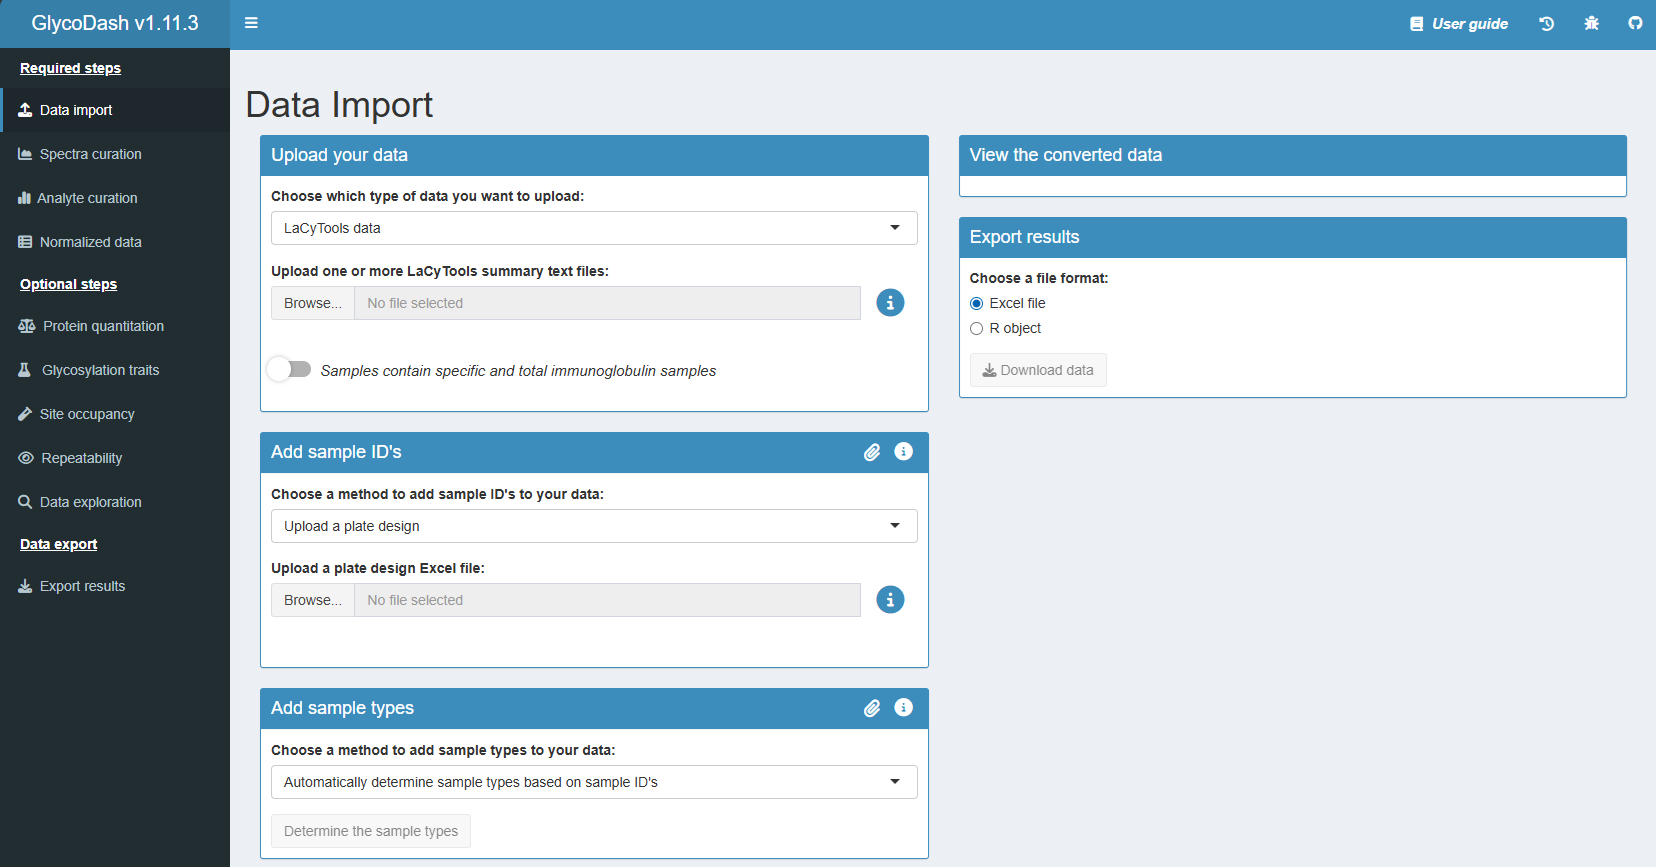
\includegraphics[scale=0.35]{interface.png}
\end{center}

The top-left corner displays the version number of GlycoDash.
The left column contains various tabs. 
The first four tabs (\menu{Data import}, \menu{Spectra curation}, \menu{Analyte curation} and \menu{Normalized data}) should be completed in the listed order, as detailed in subsequent sections. 
Later tabs are optional and can be skipped. 
The buttons in the top-right corner can be used to download the latest version of the user guide, to download a changelog, to view a list of known bugs and issues, or to visit the \href{https://github.com/Center-for-Proteomics-and-Metabolomics/GlycoDash}{GitHub page} containing the source code of GlycoDash.
